\documentclass[english, 10pt]{report}

\usepackage[T1]{fontenc}
\usepackage[latin9]{inputenc}
\usepackage{verbatim}
\usepackage{babel}
\usepackage{multirow}
\usepackage{graphicx}
\usepackage{xcolor}
\usepackage{moreverb}

%
% Listings to view code
%

\usepackage{listings}
\usepackage{courier}
 \lstset{
         basicstyle=\footnotesize\ttfamily, % Standardschrift
         %numbers=left,               % Ort der Zeilennummern
         numberstyle=\tiny,          % Stil der Zeilennummern
         %stepnumber=2,               % Abstand zwischen den Zeilennummern
         numbersep=5pt,              % Abstand der Nummern zum Text
         tabsize=2,                  % Groesse von Tabs
         extendedchars=true,         %
         breaklines=true,            % Zeilen werden Umgebrochen
         keywordstyle=\color{red},
    		frame=b,         
 %        keywordstyle=[1]\textbf,    % Stil der Keywords
 %        keywordstyle=[2]\textbf,    %
 %        keywordstyle=[3]\textbf,    %
 %        keywordstyle=[4]\textbf,   \sqrt{\sqrt{}} %
         stringstyle=\color{white}\ttfamily, % Farbe der String
         showspaces=false,           % Leerzeichen anzeigen ?
         showtabs=false,             % Tabs anzeigen ?
         xleftmargin=17pt,
         framexleftmargin=17pt,
         framexrightmargin=5pt,
         framexbottommargin=4pt,
         %backgroundcolor=\color{lightgray},
         showstringspaces=false      % Leerzeichen in Strings anzeigen ?        
 }
 \lstloadlanguages{% Check Dokumentation for further languages ...
         %[Visual]Basic
         %Pascal
         %C
         C++
         %XML
         %HTML
         %Java
 }
    %\DeclareCaptionFont{blue}{\color{blue}} 

  %\captionsetup[lstlisting]{singlelinecheck=false, labelfont={blue}, textfont={blue}}
  \usepackage{caption}
\DeclareCaptionFont{white}{\color{white}}
\DeclareCaptionFormat{listing}{\colorbox[cmyk]{0.43, 0.35, 0.35,0.01}{\parbox{\textwidth}{\hspace{15pt}#1#2#3}}}
\captionsetup[lstlisting]{format=listing,labelfont=white,textfont=white, singlelinecheck=false, margin=0pt, font={bf,footnotesize}}

%
% End Listings
%

\begin{document}

\title{Diploma Thesis}


\author{Andreas Gruber}
\maketitle
\begin{abstract}
The amount of robots in our life rises very fast. They build our cars,
they mow the lawn, they do the hoovering and a lot of other things
which most people do not even recognize. Most of these intelligent
systems which are mobile systems, are connected to a central control
station or are remotely controlled. In some cases, however, it is
impossible to connect the mobile system to a control device or the
mobile system needs to act very fast and, therefore, needs to calculate
its behaviour by its own. In this case a device needs to know  its
current position, speed, and direction. Also a lot of other properties
need to be known to compute a behaviour which is as good as possible
for the current situation. To find out the values of these properties
the robot needs a lot of sensors. In order to keep the production
costs low, the mass of these sensors is pretty cheap which, in turn,
rises the problem that those can produce errors and they even can
brake while the device is working. In one of these cases the device
should detect that the sensor doesn't work any more and replace its
results by the result of other sensors.

The main goal of this thesis is to build a system which calculates the
most accurate current position of a model car based on a set of different
(cheap) sensors. To take more cheap sensors
has a lot of pros. First the whole device can be produced very cheaply.
Another very important consequence is that other cheap sensors help
to improve the results. The most important advantage (??) is that
errors and measuring faults can be detected and the wrong values can
be replaced by correct ones. Systems like this have a big application
spectrum in future because autonomous robots will be needed in more
and more branches.

Write about three sentences about the co-operation with FLLL in Hagenberg.\end{abstract}
\begin{itemize}
\item There is a co-operation, who is the contact person
\item What is the FLLL working in?
\item What is the general project you are working in? How does your thesis
fit into the general work of the FLLL?\end{itemize}

\tableofcontents

\chapter{Environment}
\section{AVR}
AVR is the name of a microcontroller-family which is produces by the company Atmel.
Atmel produces different types of microcontroller.
The different types can be grouped in:\\
\\
\begin{tabular}{ll}
32-bit AVR UC3		&										\\
AVR XMEGA			&										\\
Automotive AVR		&										\\
megaAVR			& 										\\
tinyAVR			& (Small, cheap microcontroller with a power supply down to 0,7 V)\\
Battery Management	& (Battery management chips for Li-ion batteries)			\\
\end{tabular}
\\
During this diploma thesis I mostly using megaAVR or ATmega.

\subsection{ATmega 2560}
ATmega 2560 is part of many different electronic projects.
It is a very powerful microcontroller wich has a lot of different hardware implemented features.
\subsubsection{Summary}
\begin{tabular}{ll}
Speed Grade		& 0-16 MHz	\\
Flash Memory	& 256 KB	\\
SRAM			& 8 KB		\\
EEPROM		& 4 KB		\\
I/O Lines		& 86		\\
8-bit Timer		& 2		\\
16-bit Timer		& 4		\\
4-bit PWM		& 4		\\
2 to 16-bit PWM	& 12		\\
10-bit ADC		& 16		\\
USART / UART	& 4		\\
TWI / I2C		& 1		\\
\end{tabular}

\section{Arduino}
\subsection{Arduino Mega 2560}
\makebox[\linewidth]{
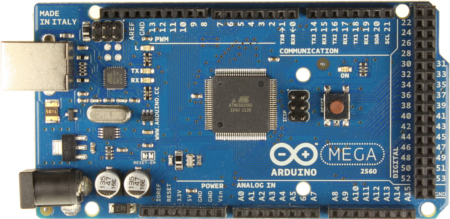
\includegraphics[width=0.8\textwidth]{img_ArduinoMega2560_R3_Front_450px.jpg}
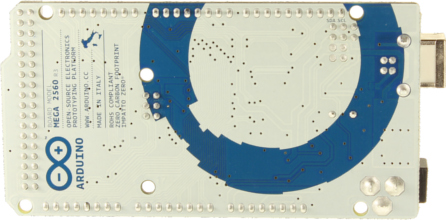
\includegraphics[width=0.8\textwidth]{img_ArduinoMega2560_R3_Back_450px.jpg}
}
\\
The Arduino Mega 2560 is a microcontroller board based on the ATmega 2560.
It contains the full hardware to programm the microcontroller.
So a USB to serial converter is installed on the board.
The board also contains also a voltage regulator to supply it by an external power supply
\\
The design has the advantage that the shields from the Arduino UNO are compatible to the Arduino Mega

\subsection{Datatypes}
\makebox[\linewidth]{
\begin{tabular}{|l|r|c|c|r|r|}
\hline
\multirow{2}{*}{data type} & \multirow{2}{*}{Bit} & \multicolumn{4}{|c|}{value}  \\
\cline{3-6}
& & min & max & min & max \\
\hline
int8\_t, signed char				& $8$		& $-128$				& $127$				& $-2^{7}$		& $2^{7}-1$		\\
int16\_t, signed short, signed int		& $16$	& $-32768$				& $32767$				& $-2^{15}$		& $2^{15}-1$	\\
int32\_t, signed long			& $32$ 	& $-2147483648$			& $2147483647$			& $-2^{31}$		& $2^{31}-1$	\\
int64\_t, signed long long			& $64$ 	& $-9223372036854775808$	& $9223372036854775807$	& $-2^{63}$		& $2^{63}-1$	\\
& & & & & \\
uint8\_t, unsigned char			& $8$		& $0$					& $255$				& $0$			& $2^{8}-1$		\\
uint16\_t, unsigned short, unsigned int	& $16$ 	& $0$					& 65535				& $0$ 			& $2^{16}-1$	\\
uint32\_t, unsigned long			& $32$ 	& $0$					& $4294967295$			& $0$			& $2^{32}-1$	\\
uint64\_t, unsigned long long		& $64$ 	& $0$					& $18446744073709551615$	& $0$			& $2^{64}-1$	\\
& & & & & \\
float, double					& $32$ 	& $-3.4028235*10^{38}$		& $3.4028235*10^{38}$		&			&			\\
\hline
\end{tabular}
}


\subsection{Microcontroller I/O}
\subsubsection{Digital input Pins}
\lstinline|value = digitalRead(pin)|

\subsubsection{Digital output Pins}
\lstinline|digitalWrite(pin, value)|

\subsubsection{Analog inupt Pins}
\lstinline|value = analogRead(Apin)| \\
Value has a resolution of 10 Bit.
So analog read will return a value between 0 and 1024.

\subsubsection{Analog Output / PWM Pins}
\lstinline|analogWrite(PWMpin, value)| \\
Value have to be between 0 (off) and 255 (on)

\subsubsection{UART}
Before the serial connection is used it have to be started: \\
\lstinline|Serial.beginn(speed);| \\
Then bytes can be written to ther serial port: \\
\lstinline|Serial.write(value);| \\
Or something can be printed to the serial port: \\
\lstinline|Serial.println(value);| \\
A small code snippet for a serial connection could look like this:\\
\begin{lstlisting}
Serial.beginn(9600);
Serial.println("Hello World");
byte in;
while(Serial.available() > 0)
	in = Serial.read();
char c = Serial.read();
\end{lstlisting}

\subsubsection{I2C}
At first the I2C bus have to be started: \\
\lstinline|Wire.beginn(address);| \\
Then a request can be started: \\
\lstinline|Wire.requestFrom(device,size);| \\
At least bytes can be read from the device: \\
\lstinline|byte b = Wire.read();| \\
Another option is to start a transmission:\
\lstinline|Wire.beginTransmission(device);| \\
Then it is possible to write data to the communication partner:\\
\lstinline|Wire.write(value);|\\
After sending the data the transmmission have to be closed:\\
\lstinline|Wire.endTransmission();|\\
A example for a I2C connection could look like this:\\
\begin{lstlisting}
Wire.begin()
Wire.requestFrom(0x23,1);
byte b = Wire.read();
Wire.beginTransmission(0x23);
Wire.write(b);
Wire.endTransmission();
\end{lstlisting}


\end{document}



















